\documentclass[12pt]{report}


% includes
\usepackage{geometry}           % page size
\usepackage[utf8]{inputenc}     % encoding
\usepackage{palatino}           % font
\usepackage[romanian]{babel}    % language
\usepackage{graphicx}           % images
\usepackage{listings}
\usepackage{indentfirst}        % indentation
\usepackage[nottoc]{tocbibind}  % table of contents style
\usepackage[unicode]{hyperref}  % references from the table of contents
\usepackage[numbers]{natbib}
\usepackage{url}
\usepackage{hyperref}

\usepackage{listings}
\usepackage{color}
 
\bibliographystyle{ieeetr}

\lstloadlanguages{[Sharp]C,C++,csh,Java}

\definecolor{red}{rgb}{0.6,0,0} 
\definecolor{blue}{rgb}{0,0,0.6}
\definecolor{green}{rgb}{0,0.8,0}
\definecolor{mauve}{rgb}{0.5,0.05,0.5}
\definecolor{cloudwhite}{rgb}{0.97,0.96,0.94}



% includes options
\geometry{  a4paper,            % scientific thesis standard
            left=3cm,
            right=2cm,
            top=2cm,
            bottom=2cm,
 }
\graphicspath{{images/}}        % path where the images are located
\setlength{\parindent}{1cm}     % paragraph indentation

% other options
\linespread{1.5}                % space between lines
\renewcommand*\contentsname{Cuprins}    % table of contents name
\let\cite\citep
% the document content
\begin{document}


\lstset{
language=csh,
basicstyle=\footnotesize\ttfamily,
numbers=left,
numberstyle=\tiny,
tabsize=2,
breaklines=true,
frame=b,
showspaces=false,
showtabs=false,
commentstyle=\color{green},
keywordstyle=\color{mauve},
morekeywords={lemma, method, function, predicate,ensures, requires, assert },
identifierstyle=\color{black},
backgroundcolor=\color{cloudwhite},
}


    % macros (global)
    \newcommand{\university}    {Universitatea "Alexandru-Ioan Cuza" din Iași}
\newcommand{\universityg}   {Universității "Alexandru-Ioan Cuza" din Iași} % genitive
\newcommand{\faculty}       {Facultatea de informatică}
\newcommand{\facultyg}      {Facultății de informatică} % genitive
\newcommand{\speciality}    {informatică}
\newcommand{\promotion}     {2022}                                  %<---------

\newcommand{\thesistype}    {Lucrare de licență}
\newcommand{\thesistitle}   {Implementarea și verificarea formală în Dafny a algoritmului greedy pentru o variantă a problemei bancnotelor}    %<---------

\newcommand{\authorlast}    {Contur}                               %<---------
\newcommand{\authorfirst}   {Alexandra Elena}
\newcommand{\authornamefl}  {\authorfirst \space \authorlast} % first name first
\newcommand{\authornamelf}  {\authorlast \space \authorfirst} % last name first
\newcommand{\authorbirth}   {04 martie 2001}                      %<---------
\newcommand{\authoraddress} {România, jud. Iași, com. Holboca, str. Dascălilor, nr. 10} %<---------
\newcommand{\authorcnp}     {6010304226743}                         %<---------

\newcommand{\session}       {februarie, 2023}                       %<---------
\newcommand{\coordinator}   {Conf. Dr. Ciobâcă Ștefan}               %<---------

\newcommand{\dottedline}    {............................}
    
    % front-matter
    \pagenumbering{gobble}
    
    % define the cover page
\begin{titlepage}
    \begin{center}
        % the university and faculty
        \large
        \MakeUppercase{\university}
        
        \LARGE
        \textbf{\MakeUppercase{\faculty}}
        
        % the faculty logo
        \vspace{1cm}
        
\includegraphics[width=0.3\textwidth]{logoFii.png}
        
        % thesis title
        \vspace{1cm}
        \Large
        \MakeUppercase{\thesistype}
        
        \vspace{0.5cm}
        \LARGE
        \textbf{\thesistitle}
        
        % author
        \vspace{2cm}
        \Large
        propusă de
        
        \vspace{0.5cm}
        \LARGE
        \textbf{\authornamefl}
        
        % session
        \vfill
        \Large
        \textbf{Sesiunea:} \session
        
        % scientific coordinator
        \vspace{2cm}
        \Large
        Coordonator științific
        
        \vspace{0.5cm}
        \LARGE
        \textbf{\coordinator}
    \end{center}
\end{titlepage}
    % define the title page
\begin{titlepage}
    \begin{center}
        % the university and faculty
        \large
        \MakeUppercase{\university}
        
        \LARGE
        \textbf{\MakeUppercase{\faculty}}
        
        % thesis title
        \vspace{5cm}
        \huge
        \textbf{\thesistitle}
        
        % author
        \vspace{2cm}
        \LARGE
        \textbf{\authornamefl}
        
        % session
        \vfill
        \Large
        \textbf{Sesiunea:} \session
        
        % scientific coordinator
        \vspace{4cm}
        \Large
        Coordonator științific
        
        \vspace{0.5cm}
        \LARGE
        \textbf{\coordinator}
    \end{center}
\end{titlepage}
    \vspace*{\fill}

\begin{flushright}
    Avizat, \\
    Îndrumător lucrare de licență, \\
    \coordinator. \\
    Data: \dottedline \hspace{1cm} Semnătura: \dottedline
\end{flushright}

\vspace{1cm}
\begin{center}
    \large
    \textbf{Declarație privind originalitatea conținutului lucrării de licență}
\end{center}

Subsemnatul \textbf{\authornamelf} domiciliat în \textbf{\authoraddress}, născut la data de \textbf{\authorbirth}, identificat prin CNP \textbf{\authorcnp}, absolvent al \facultyg, \textbf{\faculty} specializarea \textbf{\speciality}, promoția \promotion, declar pe propria răspundere cunoscând consecințele falsului în declarații în sensul art. 326 din Noul Cod Penal și dispozițiile Legii Educației Naționale nr. 1/2011 art. 143 al. 4 și 5 referitoare la plagiat, că lucrarea de licență cu titlul \textbf{\thesistitle} elaborată sub îndrumarea domnului \textbf{\coordinator}, pe care urmează să o susțin în fața comisiei este originală, îmi aparține și îmi asum conținutul său în întregime.

De asemenea, declar că sunt de acord ca lucrarea mea de licență să fie verificată prin orice modalitate legală pentru confirmarea originalității, consimțind inclusiv la introducerea conținutului ei într-o bază de date în acest scop.

Am luat la cunoștință despre faptul că este interzisă comercializarea de lucrări științifice în vederea facilitării falsificării de către cumpărător a calității de autor al unei lucrări de licență, de diplomă sau de disertație și în acest sens, declar pe proprie răspundere că lucrarea de față nu a fost copiată ci reprezintă rodul cercetării pe care am întreprins-o.

\begin{flushright}
    Data: \dottedline \hspace{6cm} Semnătura: \dottedline
\end{flushright}

\vspace*{\fill}
\pagebreak
    \vspace*{\fill}
\begin{center}
    \large
    \textbf{Declarație de consimțământ}
\end{center}

Prin prezenta declar că sunt de acord ca lucrarea de licență cu titlul \textbf{\thesistitle}, codul sursă al programelor și celelalte conținuturi (grafice, multimedia, date de test, etc.) care însoțesc această lucrare să fie utilizate în cadrul \facultyg.

De asemenea, sunt de acord ca \faculty \space de la \university, să utilizeze, modifice, reproducă și să distribuie în scopuri necomerciale programele-calculator, format executabil și sursă, realizate de mine în cadrul prezentei lucrări de licență.

\begin{flushright}
    Absolvent \textbf{\authornamefl} \\
    \vspace{0.5cm}
    Data: \dottedline \hspace{6cm} Semnătura: \dottedline
\end{flushright}
\vspace*{\fill}
\pagebreak
    
    % table of contents
    \tableofcontents
    
    % chapters
    \setcounter{page}{1}
    \pagenumbering{arabic}
    
    
\chapter{Context} 

 
Dafny este un limbaj de programare și verificare, capabil să verifice corectitudinea
funcțională a unui program.\par
Verificarea este posibilă datorită caracteristicilor specifice limbajului precum precondiții, postcondiții, 
invariante, ș.a.m.d. De asemenea, verificatorul Dafny are grijă ca adnotările făcute să se îndeplinească,
astfel acesta ne scapă de povara de a scrie cod fără erori, în schimbul scrierii de adnotări fără erori.
 
Problema bancnotelor are ca scop reprezentarea unei sume într-un număr minim posibil de bancnote.\par
Metoda greedy face alegerea cea mai bună la fiecare pas, construind soluția finală.
Verificarea formală in Dafny a problemei bancnotelor demonstrează faptul că soluția construită este optimă
pentru orice sumă dată ca input. \par
Reprezentarea folosită pentru soluție este :
$ banknote_{1}:= 1 < banknote_{2} < ... < banknote_{n} $. 

Anterior am menționat forma generală a problemei bancnotelor.\par
Bancnotele posibile în problema bancnotelor cu $2^{5}$ sistem de bancnote sunt: 
$[1, 2, 4, 8, 16, 32]$ . 

Datorită bancnotelor care sunt puteri ale lui 2, dacă avem mai mult de o bancnotă de valoare mai mică decât 32,
putem înlocui 2 bancnote de acea valoare cu o bancnotă de valoarea următoare și am obține o soluție cu cost mai mic.\par
Astfel, am descoperit proprietatea: 
$  forall$ $i :: 0 <= i <= 4 ==> s[i] <= 1 $


    \chapter{Reprezentarea problemei în Dafny}


\section{ Reprezentarea datelor de intrare }
În cazul problemei discutate datele de intrare sunt reprezentate de o variabilă \textbf{sum} ce reprezintă
 suma pentru care se verifică dacă se produce soluția finală.

\section{ Reprezentarea datelor de ieșire}
Datele de ieșire sunt reprezentate de o secvență de forma : \par
$\bullet$ soluție  = { $b_{0}, b_{1}, b_{2}, b_{3}, b_{4}, b_{5}$} , unde $\sum_{k=0}^{5} b_{k} \cdot 2^{k} = suma $

\section{ Structuri de date folosite}
-solutia reprezentata ca secventa
-cele 3 predicate explicate + exemple cod
\subsection{Condiții ca o soluție finală să fie optimă}
    $\bullet$ Pentru a avea o soluție optimă trebuie să avem o soluție validă (cu 6 elemente), care produce suma corectă
     și care are costul cel mai mic.\par
    $\bullet$ Pentru a avea o soluție optimă finală, pe parcursul construirii soluției, în buclă, trebuie menținută proprietatea
     de a alege soluția optimă locală pentru rest, iar suma soluțiilor optime locale să fie soluție optimă pentru sumă.\par
    $\bullet$ Soluția formată dintr-o bancnotă, cea aleasă în iterația curentă, produce o soluție optimă pentru suma 
    de valoare bancnotă, asigurând faptul că avem o soluție optimă locală.\par
    $\bullet$ O soluție optimă pentru suma $x$, adunată cu o soluție optimă pentru suma $y$ creează o soluție optimă pentru suma $x+y$, 
    asigurând faptul că suma soluțiilor locale creează soluția finală optimă.\par
    
    
\lstset{
language=csh,
basicstyle=\footnotesize\ttfamily,
numbers=left,
numberstyle=\tiny,
tabsize=2,
breaklines=true,
frame=b,
showspaces=false,
showtabs=false,
commentstyle=\color{green},
keywordstyle=\color{mauve},
morekeywords={lemma, method, function, predicate,ensures, requires, assert },
identifierstyle=\color{black},
backgroundcolor=\color{cloudwhite},
}

\chapter{Verificarea formală a problemei}

\section{Implementarea algoritmului}
    Implementarea algoritmului propriu-zis care rezolvă problema a fost primul și cel mai ușor pas.\par
    Am început prin crearea unei bucle care la fiecare pas alegea bancnota optimă, o adăuga în secvența de 
    bancnote considerată soluție și o scădea din sumă, fiind un algoritm tipic metodei Greedy.
    \begin{lstlisting}
    var rest:= sum;
    solution:= [0, 0, 0, 0, 0, 0];
    while (0 < rest)
        decreases rest 
        {
        index:= maxBanknote(rest);
        var banknote:= power(2, index);
        solution:= addValueToIndex(solution,1,index);
        rest:= rest - banknote;
    }
    \end{lstlisting}

    Acest algoritm era suficient pentru a rezolva problema, dar nu era suficient pentru a demonstra că soluția produsă este optimă.\par
    Considerăm o soluție optimă soluția de cost minim, costul fiind numărul de bancnote.
    
\section{Demonstrarea optimalității}
    \subsection{Schema verificării}
    \vspace{1cm}
    \begin{center}
        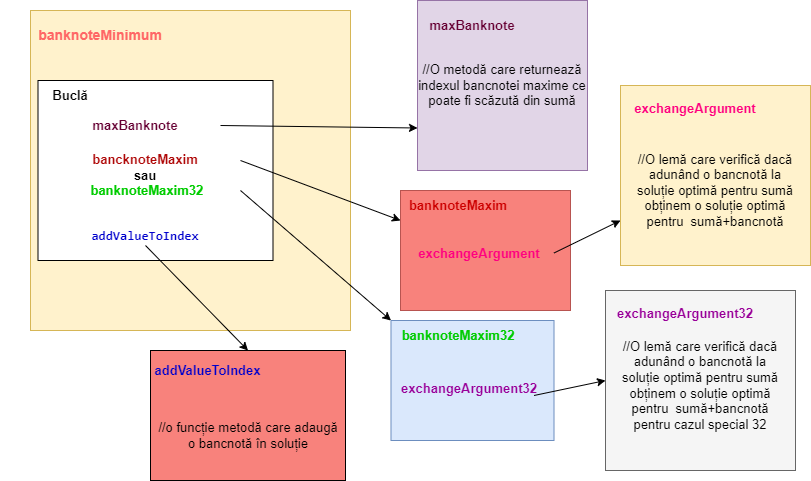
\includegraphics[width=1.0\textwidth]{verification_schema.png}\par
    \end{center}
    În schema de mai sus am exemplificat modul în care funcțiile, lemele și metodele se apelează una pe cealaltă pentru a demonstra faptul că soluția găsită este soluție optimă.\par

    \subsection{Condiții ca o soluția finală să fie optimă}
    $\bullet$ Pentru a avea o soluție optimă trebuie să avem o soluție validă (cu 6 elemente), care produce suma corectă
     și care are costul cel mai mic.\par
    $\bullet$ Pentru a avea o soluție optimă finală, pe parcursul construirii soluției, în buclă, trebuie menținută proprietatea
     de a alege soluția optimă locală pentru rest, iar suma soluțiilor optime locale să fie soluție optimă pentru sumă.\par
    $\bullet$ Soluția formată dintr-o bancnotă, cea aleasă în iterația curentă, produce o soluție optimă pentru suma 
    de valoare bancnotă, asigurând faptul că avem o soluție optimă locală.\par
    $\bullet$ O soluție optimă pentru suma $x$, adunată cu o soluție optimă pentru suma $y$ creează o soluție optimă pentru suma $x+y$, 
    asigurând faptul că suma soluțiilor locale creează soluția finală optimă.\par
    
\section{Pașii verificării}
    \subsection{banknoteMinimum}
    Am implementat algoritmul Greedy care rezolva Problema Bancnotelor cu bancnote puteri ale lui 2, 
    apoi am adăugat treptat condițiile care garantează că soluția găsită este soluție optimă.\par
    \begin{lstlisting}
    method banknoteMinimum(sum: int) returns(solution: seq < int > )
        requires sum >= 0
        ensures isValidSolution(solution)
        ensures isSolution(solution, sum)
        ensures isOptimalSolution(solution, sum) 
    {
        var rest:= sum;
        solution:= [0, 0, 0, 0, 0, 0];
        var index:= 0;
        assert isOptimalSolution(solution, sum - rest);
        while (0 < rest)
            invariant 0 <= rest <= sum
            invariant isValidSolution(solution)
            invariant addOptimRestEqualsOptimSum(rest, sum, solution)
            decreases rest 
        {
            index:= maxBanknote(rest);
            var banknote:= power(2, index);
            if (index != 5) 
            {
                banknoteMaxim(rest, sum, solution, index);
            } 
            else 
            {
                banknoteMaxim32(rest, sum, solution);
            }
            solution:= addValueToIndex(solution,1,index);
            rest:= rest - banknote;
        }
    }
    \end{lstlisting}
    \subsection{maxBanknote}
    Pentru a alege bancnota cea mai mare am creat funcția maxBanknote.\par
    \begin{lstlisting}
      method maxBanknote(sum: int) returns(index: int)
        requires sum > 0
        ensures 0 <= index <= 5
        ensures 0 <= power(2, index) <= sum
        ensures(index != 5 && power(2, index + 1) > sum) || index == 5 
      {
        index:= 5;
        if (power(2, index) > sum) 
        {
          assert power(2, index + 1) > sum;
          while (power(2, index) > sum && index > 0)
            invariant power(2, index + 1) > sum 
            {
              index:= index - 1;
              assert power(2, index + 1) > sum;
            }
        } 
          else 
        {
          assert index == 5;
        }
      }
    \end{lstlisting}


    \subsection{banknoteMaxim}
    Metoda maxBanknote este folosită pentru a returna un index cu proprietatea: \par
     $bancnota_{index} <= rest < bancnota_{index + 1}$  .
    \begin{lstlisting}
    lemma banknoteMaxim(rest: int, sum: int, finalSolution: seq < int > , index: int)
        requires 0 <= index <= 4
        requires power(2, index) <= rest < power(2, index + 1)
        requires isValidSolution(finalSolution)
        requires addOptimRestEqualsOptimSum(rest, sum, finalSolution)
        ensures addOptimRestEqualsOptimSum(rest - power(2, index), sum, finalSolution[index:= finalSolution[index] + 1]) 
    {
        var banknote:= power(2, index);
        forall currentSolution | isValidSolution(currentSolution) && isOptimalSolution(currentSolution, rest - banknote)
            ensures isOptimalSolution(solutionsSum(solutionsSum(currentSolution, finalSolution), [0, 0, 0, 0, 0, 0][index:= 1]), sum) 
        {
            assert isSolution(currentSolution[index:= currentSolution[index] + 1], rest);
            exchangeArgument(rest, currentSolution, index);
        }
        assert forall currentSolution::isValidSolution(currentSolution) && isOptimalSolution(currentSolution, rest - banknote) ==> isOptimalSolution(solutionsSum(solutionsSum(currentSolution, finalSolution), [0, 0, 0, 0, 0, 0][index:= 1]), sum);
    }
    \end{lstlisting}

    \subsection{exchangeArgument}
    \begin{lstlisting}
        lemma exchangeArgument(rest: int, currentSolution: seq < int > , index: int)
            requires 0 <= index <= 4
            requires power(2, index) <= rest < power(2, index + 1)
            requires isValidSolution(currentSolution)
            requires isOptimalSolution(currentSolution, rest - power(2, index))
            ensures isOptimalSolution(currentSolution[index:= currentSolution[index] + 1], rest) 
        {
            var banknote:= power(2, index);
            var solution:= currentSolution[index:= currentSolution[index] + 1];
            assert isValidSolution(solution);
            assert isSolution(solution, rest);
            var i:= index;
            if (!isOptimalSolution(solution, rest)) 
            {
            var optimalSolution:| isValidSolution(optimalSolution) && isSolution(optimalSolution, rest) &&
                isOptimalSolution(optimalSolution, rest) && cost(optimalSolution) < cost(solution);

            assert cost(solution) == cost(currentSolution) + 1;
            assert isOptimalSolution(optimalSolution, rest);

            if (optimalSolution[index] -1 >= 0) 
            {
                assert optimalSolution[index]-1 >= 0;
                var betterSolution:= addValueToIndex(optimalSolution,-1,index);
                assert isSolution(betterSolution, rest - banknote);
                assert cost(betterSolution) == cost(optimalSolution) - 1;
                assert cost(optimalSolution) - 1 < cost(currentSolution);
                assert false;
            } 
            else 
            {
                while (0 < i)
                invariant 0 <= i <= index
                invariant forall x::index >= x >= i ==> optimalSolution[x] <= 1 
                {
                i:= i - 1;
                assert isOptimalSolution(optimalSolution, rest);
                if (optimalSolution[i] > 1) 
                {
                    var optimalSolution' := optimalSolution[i:=optimalSolution[i]-2];
                    optimalSolution' := optimalSolution' [i + 1:= optimalSolution'[i+1]+1];
                    assert isSolution(optimalSolution', rest);
                    assert cost(optimalSolution') == cost(optimalSolution) - 1;
                    assert cost(optimalSolution') < cost(optimalSolution);
                    assert false;
                }
                }
                assert solutionElementsSum(optimalSolution) <= banknote - 1; assert rest >= banknote; assert solutionElementsSum(optimalSolution) <= rest - 1; assert isOptimalSolution(optimalSolution, rest); assert false;
            }
            }
        }
    \end{lstlisting}

    \subsection{addValueToIndex}
    \begin{lstlisting}
        function method addValueToIndex(solution: seq<int>, value: int, index: int): seq<int>
            requires 0 <= index <= 5
            requires isValidSolution(solution)
            requires solution[index] + value >= 0
            ensures isValidSolution(solution)
            ensures solutionElementsSum(solution) + value*power(2, index) == solutionElementsSum(solution[index:=solution[index]+value])
        {
        solution[index:= solution[index] + value]
        }
    \end{lstlisting}

    
    \subsection{Ultimul pas}
    În final, am descoperit că pentru bancnota 32 am nevoie de o verificare diferită. Voi descrie ulterior cum am tratat acest caz.\par
    $\bullet$ De ce trebuie abordat diferit cazul când bancnota optimă de adăugat este 32?\par
    Fiecare bancnotă 1,2,4,8 și 16 este mărginită superior de bancnota imediat următoare, datorită felului în care 
    se alege index-ul în metoda maxBanknote.\par
    Felul în care abordez cazurile 1,2,4,8 și 16 constă în verificarea faptului că 
    nu avem încă o bancnotă de aceeași valoare în soluție deja, altfel ar fi mai eficient să avem  
    o bancnotă de valoarea imediat următoare și să scăpăm de bancnota deja existentă din soluție.\par
    În cazul bancnotei 32 nu există o altă bancnotă de valoare mai mare cu care putem să înlocuim apariția bancnotei 32,
    așadar a trebuit să demonstrez că adăugând bancnota 32 la soluția găsită până în prezent se generează o soluție optimă pentru 
    pentru restul dat până în prezent.   
    
    
    
    
\section{Problema bancnotei nemărginite superior, 32}

\subsection{Cum se tratează separat cazul 32}

\subsection{banknoteMaxim32}
\begin{lstlisting}
lemma banknoteMaxim32(rest: int, sum: int, finalSolution: seq < int > )
  requires rest >= 32
  requires isValidSolution(finalSolution)
  requires addOptimRestEqualsOptimSum(rest, sum, finalSolution)
  ensures addOptimRestEqualsOptimSum(rest - 32, sum, solutionsSum(finalSolution, [0, 0, 0, 0, 0, 1])) 
{
  forall currentSolution | isValidSolution(currentSolution) && isSolution(currentSolution, rest - 32)
    ensures isSolution(solutionsSum(solutionsSum(finalSolution, currentSolution), [0, 0, 0, 0, 0, 1]), sum) 
  {
    assert isSolution(solutionsSum(currentSolution, [0, 0, 0, 0, 0, 1]), rest);
  }

  forall currentSolution | isValidSolution(currentSolution) && isOptimalSolution(currentSolution, rest - 32)
    ensures isOptimalSolution(solutionsSum(solutionsSum(finalSolution, currentSolution), [0, 0, 0, 0, 0, 1]), sum)
  {
    forall someSolution | isValidSolution(someSolution) && isSolution(someSolution, sum)
      ensures cost(someSolution) >= cost(solutionsSum(solutionsSum(finalSolution, currentSolution), [0, 0, 0, 0, 0, 1])) 
    {
      currentSolutionHasCostMin(rest, sum, currentSolution);
    }
  }
}
\end{lstlisting}

\subsection{currentSolutionHasCostMin}
\begin{lstlisting}
    lemma currentSolutionHasCostMin(rest: int, sum: int, solution: seq < int > )
  requires isValidSolution(solution)
  requires rest >= 32
  requires isSolution(solution, rest - 32)
  requires isOptimalSolution(solution, rest - 32)
  ensures isOptimalSolution(solutionsSum(solution, [0, 0, 0, 0, 0, 1]), rest) 
{
  forall someSolution | isValidSolution(someSolution) && isSolution(someSolution, rest)
    ensures cost(someSolution) >= cost(solutionsSum(solution, [0, 0, 0, 0, 0, 1])) 
  {
    exchangeArgument32(rest, sum, someSolution, solution);
  }
}

\end{lstlisting}


\subsection{exchangeArgument32}
\begin{lstlisting}
    
lemma exchangeArgument32(rest: int, sum: int, currentSolution: seq < int > , optimalSolution: seq < int > )
    requires 32 <= rest
    requires isValidSolution(optimalSolution)
    requires isOptimalSolution(optimalSolution, rest - 32)
    ensures isOptimalSolution(optimalSolution[5:= optimalSolution[5] + 1], rest) 
{
    var solution:= optimalSolution[5:= optimalSolution[5] + 1];
    var i:= 4;
    if (!isOptimalSolution(solution, rest)) 
    {
        if (optimalSolution[i] > 1) 
        {
            var solution:= optimalSolution[i:= optimalSolution[i] - 2];
            solution:= solution[i + 1:= solution[i + 1] + 1];
            assert isSolution(solution, rest - 32);
            assert cost(solution) == cost(optimalSolution) - 1;
            assert cost(optimalSolution) - 1 < cost(solution);
            assert false;
        } 
        else
        {
            while (0 < i)
                invariant 0 <= i <= 4
                invariant forall index::4 >= index >= i ==> optimalSolution[index] <= 1 
            {
                i:= i - 1;
                if (optimalSolution[i] > 1) 
                {
                    var solution:= optimalSolution[i:= optimalSolution[i] - 2];
                    solution:= solution[i + 1:= solution[i + 1] + 1];
                    assert isSolution(solution, rest - 32);
                    assert cost(solution) == cost(optimalSolution) - 1;
                    assert cost(optimalSolution) - 1 < cost(solution);
                    assert false;
                }
                assert optimalSolution[i] <= 1;
            }
            assert solutionElementsSum(optimalSolution) <= rest - 1;
            assert isOptimalSolution(solution, rest);
            assert false;
        }
    }
}

\end{lstlisting}


    \chapter*{Concluzie} 
\addcontentsline{toc}{chapter}{Concluzii}

În cadrul acestei lucrări am realizat verificarea formală a unei implementări a metodei greedy ce rezolvă o variantă a 
problemei bancnotelor cu bancnote puteri ale lui 2.\par
Implementarea unei metode greedy ce rezolvă varianta clasică a problemei bancnotelor este deja existentă, în cadrul unei lucrări de 
licență prezentată în 2022 la Facultatea de Informatică Iași~\cite{elisa:1}.\par
Una dintre dificultățile întâlnite în acest proces a fost crearea invariantului care menține proprietatea de soluție
optimă, așa a apărut predicatul addOptimRestEqualsOptimSum.\par
Acest predicat afirmă că o soluție optimă pentru o sumă x adunată cu o soluție pentru suma y are ca rezultat o 
soluție optimă pentru suma $x+y$. Astfel, secvența ce reprezintă soluția care se construiește pe parcursul buclei 
are garanția că atât timp cât se adună cu soluții locale optime, în final, vom avea o soluție finală optimă.\par
Parcurgerea acestor etape pentru verificare m-a făcut să aprofundez noțiunea de soluție și să înțeleg în amănunt 
formarea acesteia prin metoda greedy.\par
Pe viitor îmi propun să găsesc o modalitate de a unifica metodele banknoteMaxim pentru a funcționa pentru orice caz, 
astfel optimizând viteza verificării.\par
Un alt lucru interesant de făcut în viitor, ar fi găsirea unei proprietăți care să se aplice pentru orice sistem 
de bancnote, pentru a verifica faptul că produce o soluție optimă.
 

\bibliography{citations}
\end{document}
